% Options for packages loaded elsewhere
\PassOptionsToPackage{unicode}{hyperref}
\PassOptionsToPackage{hyphens}{url}
%
\documentclass[
  ngerman,
  ignorenonframetext,
]{beamer}
\usepackage{pgfpages}
\setbeamertemplate{caption}[numbered]
\setbeamertemplate{caption label separator}{: }
\setbeamercolor{caption name}{fg=normal text.fg}
\beamertemplatenavigationsymbolsempty
% Prevent slide breaks in the middle of a paragraph
\widowpenalties 1 10000
\raggedbottom
\setbeamertemplate{part page}{
  \centering
  \begin{beamercolorbox}[sep=16pt,center]{part title}
    \usebeamerfont{part title}\insertpart\par
  \end{beamercolorbox}
}
\setbeamertemplate{section page}{
  \centering
  \begin{beamercolorbox}[sep=12pt,center]{part title}
    \usebeamerfont{section title}\insertsection\par
  \end{beamercolorbox}
}
\setbeamertemplate{subsection page}{
  \centering
  \begin{beamercolorbox}[sep=8pt,center]{part title}
    \usebeamerfont{subsection title}\insertsubsection\par
  \end{beamercolorbox}
}
\AtBeginPart{
  \frame{\partpage}
}
\AtBeginSection{
  \ifbibliography
  \else
    \frame{\sectionpage}
  \fi
}
\AtBeginSubsection{
  \frame{\subsectionpage}
}
\usepackage{amsmath,amssymb}
\usepackage{lmodern}
\usepackage{iftex}
\ifPDFTeX
  \usepackage[T1]{fontenc}
  \usepackage[utf8]{inputenc}
  \usepackage{textcomp} % provide euro and other symbols
\else % if luatex or xetex
  \usepackage{unicode-math}
  \defaultfontfeatures{Scale=MatchLowercase}
  \defaultfontfeatures[\rmfamily]{Ligatures=TeX,Scale=1}
\fi
\usetheme[]{Berkeley}
% Use upquote if available, for straight quotes in verbatim environments
\IfFileExists{upquote.sty}{\usepackage{upquote}}{}
\IfFileExists{microtype.sty}{% use microtype if available
  \usepackage[]{microtype}
  \UseMicrotypeSet[protrusion]{basicmath} % disable protrusion for tt fonts
}{}
\makeatletter
\@ifundefined{KOMAClassName}{% if non-KOMA class
  \IfFileExists{parskip.sty}{%
    \usepackage{parskip}
  }{% else
    \setlength{\parindent}{0pt}
    \setlength{\parskip}{6pt plus 2pt minus 1pt}}
}{% if KOMA class
  \KOMAoptions{parskip=half}}
\makeatother
\usepackage{xcolor}
\IfFileExists{xurl.sty}{\usepackage{xurl}}{} % add URL line breaks if available
\IfFileExists{bookmark.sty}{\usepackage{bookmark}}{\usepackage{hyperref}}
\hypersetup{
  pdftitle={Thema 2: Bayes-Modelle einer kleinen Welt},
  pdfauthor={Prof.~Sauer},
  pdflang={de-DE},
  hidelinks,
  pdfcreator={LaTeX via pandoc}}
\urlstyle{same} % disable monospaced font for URLs
\newif\ifbibliography
\usepackage{color}
\usepackage{fancyvrb}
\newcommand{\VerbBar}{|}
\newcommand{\VERB}{\Verb[commandchars=\\\{\}]}
\DefineVerbatimEnvironment{Highlighting}{Verbatim}{commandchars=\\\{\}}
% Add ',fontsize=\small' for more characters per line
\usepackage{framed}
\definecolor{shadecolor}{RGB}{248,248,248}
\newenvironment{Shaded}{\begin{snugshade}}{\end{snugshade}}
\newcommand{\AlertTok}[1]{\textcolor[rgb]{0.94,0.16,0.16}{#1}}
\newcommand{\AnnotationTok}[1]{\textcolor[rgb]{0.56,0.35,0.01}{\textbf{\textit{#1}}}}
\newcommand{\AttributeTok}[1]{\textcolor[rgb]{0.77,0.63,0.00}{#1}}
\newcommand{\BaseNTok}[1]{\textcolor[rgb]{0.00,0.00,0.81}{#1}}
\newcommand{\BuiltInTok}[1]{#1}
\newcommand{\CharTok}[1]{\textcolor[rgb]{0.31,0.60,0.02}{#1}}
\newcommand{\CommentTok}[1]{\textcolor[rgb]{0.56,0.35,0.01}{\textit{#1}}}
\newcommand{\CommentVarTok}[1]{\textcolor[rgb]{0.56,0.35,0.01}{\textbf{\textit{#1}}}}
\newcommand{\ConstantTok}[1]{\textcolor[rgb]{0.00,0.00,0.00}{#1}}
\newcommand{\ControlFlowTok}[1]{\textcolor[rgb]{0.13,0.29,0.53}{\textbf{#1}}}
\newcommand{\DataTypeTok}[1]{\textcolor[rgb]{0.13,0.29,0.53}{#1}}
\newcommand{\DecValTok}[1]{\textcolor[rgb]{0.00,0.00,0.81}{#1}}
\newcommand{\DocumentationTok}[1]{\textcolor[rgb]{0.56,0.35,0.01}{\textbf{\textit{#1}}}}
\newcommand{\ErrorTok}[1]{\textcolor[rgb]{0.64,0.00,0.00}{\textbf{#1}}}
\newcommand{\ExtensionTok}[1]{#1}
\newcommand{\FloatTok}[1]{\textcolor[rgb]{0.00,0.00,0.81}{#1}}
\newcommand{\FunctionTok}[1]{\textcolor[rgb]{0.00,0.00,0.00}{#1}}
\newcommand{\ImportTok}[1]{#1}
\newcommand{\InformationTok}[1]{\textcolor[rgb]{0.56,0.35,0.01}{\textbf{\textit{#1}}}}
\newcommand{\KeywordTok}[1]{\textcolor[rgb]{0.13,0.29,0.53}{\textbf{#1}}}
\newcommand{\NormalTok}[1]{#1}
\newcommand{\OperatorTok}[1]{\textcolor[rgb]{0.81,0.36,0.00}{\textbf{#1}}}
\newcommand{\OtherTok}[1]{\textcolor[rgb]{0.56,0.35,0.01}{#1}}
\newcommand{\PreprocessorTok}[1]{\textcolor[rgb]{0.56,0.35,0.01}{\textit{#1}}}
\newcommand{\RegionMarkerTok}[1]{#1}
\newcommand{\SpecialCharTok}[1]{\textcolor[rgb]{0.00,0.00,0.00}{#1}}
\newcommand{\SpecialStringTok}[1]{\textcolor[rgb]{0.31,0.60,0.02}{#1}}
\newcommand{\StringTok}[1]{\textcolor[rgb]{0.31,0.60,0.02}{#1}}
\newcommand{\VariableTok}[1]{\textcolor[rgb]{0.00,0.00,0.00}{#1}}
\newcommand{\VerbatimStringTok}[1]{\textcolor[rgb]{0.31,0.60,0.02}{#1}}
\newcommand{\WarningTok}[1]{\textcolor[rgb]{0.56,0.35,0.01}{\textbf{\textit{#1}}}}
\setlength{\emergencystretch}{3em} % prevent overfull lines
\providecommand{\tightlist}{%
  \setlength{\itemsep}{0pt}\setlength{\parskip}{0pt}}
\setcounter{secnumdepth}{-\maxdimen} % remove section numbering
%\setbeamertemplate{page number in head/foot}[totalframenumber]
\setbeamertemplate{footline}[frame number]
\ifXeTeX
  % Load polyglossia as late as possible: uses bidi with RTL langages (e.g. Hebrew, Arabic)
  \usepackage{polyglossia}
  \setmainlanguage[]{german}
\else
  \usepackage[main=ngerman]{babel}
% get rid of language-specific shorthands (see #6817):
\let\LanguageShortHands\languageshorthands
\def\languageshorthands#1{}
\fi
\ifLuaTeX
  \usepackage{selnolig}  % disable illegal ligatures
\fi
\newlength{\cslhangindent}
\setlength{\cslhangindent}{1.5em}
\newlength{\csllabelwidth}
\setlength{\csllabelwidth}{3em}
\newenvironment{CSLReferences}[2] % #1 hanging-ident, #2 entry spacing
 {% don't indent paragraphs
  \setlength{\parindent}{0pt}
  % turn on hanging indent if param 1 is 1
  \ifodd #1 \everypar{\setlength{\hangindent}{\cslhangindent}}\ignorespaces\fi
  % set entry spacing
  \ifnum #2 > 0
  \setlength{\parskip}{#2\baselineskip}
  \fi
 }%
 {}
\usepackage{calc}
\newcommand{\CSLBlock}[1]{#1\hfill\break}
\newcommand{\CSLLeftMargin}[1]{\parbox[t]{\csllabelwidth}{#1}}
\newcommand{\CSLRightInline}[1]{\parbox[t]{\linewidth - \csllabelwidth}{#1}\break}
\newcommand{\CSLIndent}[1]{\hspace{\cslhangindent}#1}

\title{Thema 2: Bayes-Modelle einer kleinen Welt}
\subtitle{QM2, ReThink\_v1, Kap. 2}
\author{Prof.~Sauer}
\date{WiSe 21}
\institute{AWM, HS Ansbach}

\begin{document}
\frame{\titlepage}

\begin{frame}[allowframebreaks]
  \tableofcontents[hideallsubsections]
\end{frame}
\hypertarget{kleine-welt-grouxdfe-welt}{%
\section{Kleine Welt, große Welt}\label{kleine-welt-grouxdfe-welt}}

\begin{frame}{Behaims Globus, Kolumbus glücklicher Fehler}
\protect\hypertarget{behaims-globus-kolumbus-gluxfccklicher-fehler}{}
\begin{figure}[H]
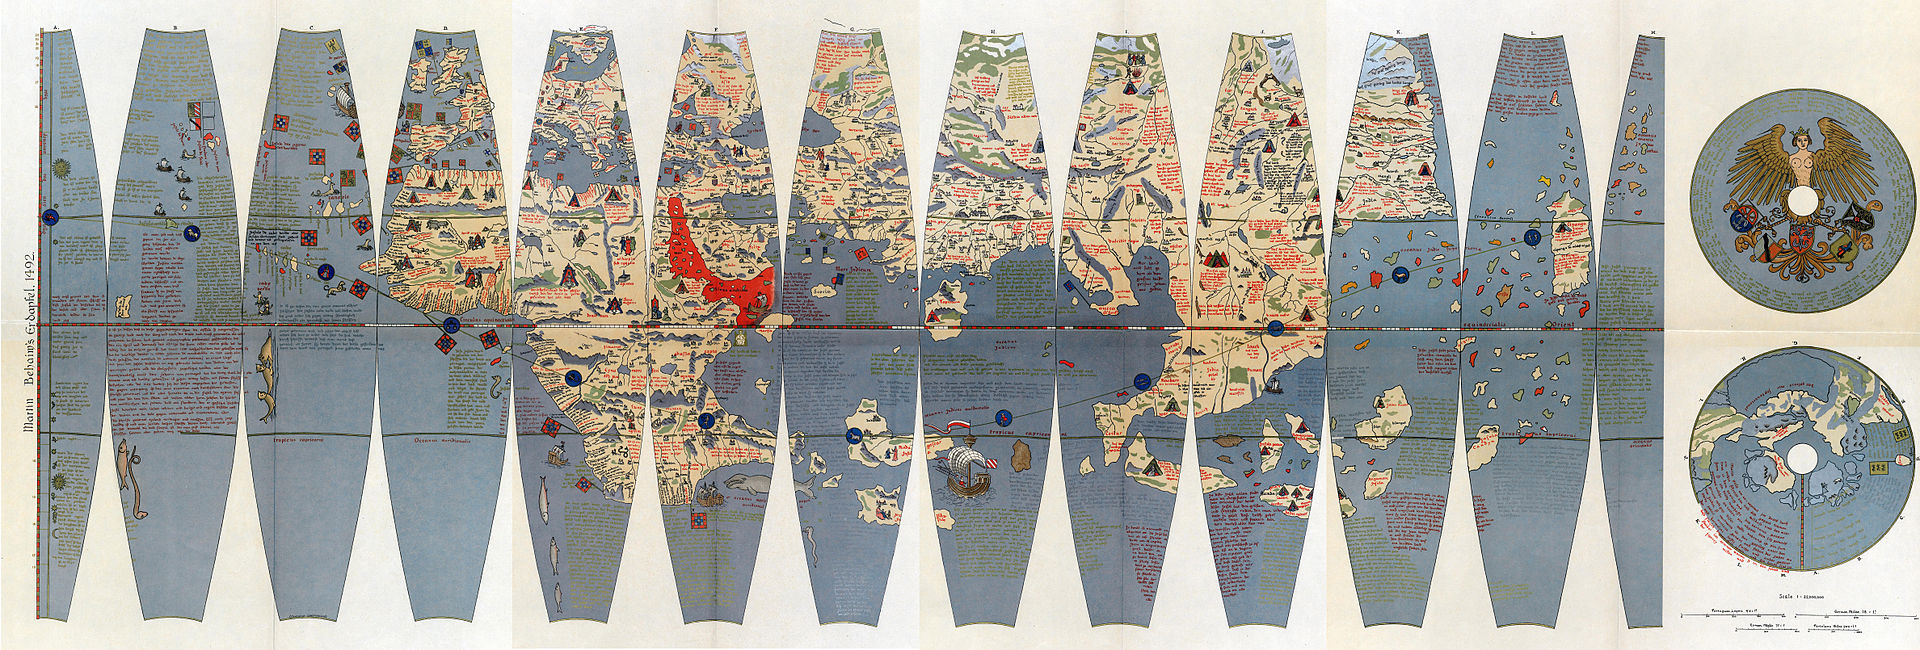
\includegraphics[width=0.7\linewidth]{img/Behaim} \end{figure}

\href{https://de.wikipedia.org/wiki/Martin_Behaims_Erdapfel\#/media/Datei:RavensteinBehaim.jpg}{Quelle}
\end{frame}

\begin{frame}{Kleine Welt, große Welt}
\protect\hypertarget{kleine-welt-grouxdfe-welt-1}{}
\begin{columns}[T]
\begin{column}{0.5\textwidth}
\begin{block}{Kleine Welt}
\protect\hypertarget{kleine-welt}{}
\begin{itemize}
\tightlist
\item
  Die Welt, wie sie der Golem sieht
\item
  entspricht dem Modell
\end{itemize}
\end{block}
\end{column}

\begin{column}{0.5\textwidth}
\begin{block}{Große Welt}
\protect\hypertarget{grouxdfe-welt}{}
\begin{itemize}
\tightlist
\item
  Die Welt, wie sie in Wirklichkeit ist
\item
  entspricht nicht (zwangsläufig) dem Modell
\end{itemize}
\end{block}
\end{column}
\end{columns}

\begin{itemize}
\tightlist
\item
  Die kleine Welt ist nicht die große Welt.
\item
  Was in der kleinen Welt funktioniert, muss nicht in der großen Welt
  funktionieren.
\item
  Modelle zeigen immer nur die kleine Welt: Vorsicht vor schnellen
  Schlüssen und vermeintlicher Gewissheit.
\end{itemize}
\end{frame}

\hypertarget{bayes-statistik-als-zuxe4hlen}{%
\section{Bayes-Statistik als
Zählen}\label{bayes-statistik-als-zuxe4hlen}}

\begin{frame}{Murmeln im Säckchen}
\protect\hypertarget{murmeln-im-suxe4ckchen}{}
\begin{itemize}
\item
  Sie haben ein Säckchen mit vier Murmeln darin.
\item
  Sie wissen nicht, welche Farben die Murmeln haben.
\item
  Murmeln gibt's in zwei Farben: weiß (W) oder blau (B).
\item
  Es gibt daher fünf \emph{Hypothesen} zur Farbe der Murmeln im
  Säckchen: WWWW, BWWW, BBWW, BBBW, BBBB.
\item
  Unsere Aufgabe ist, die Wahrscheinlichkeiten der Hypothesen nach
  Ziehen von Murmeln zu bestimmen.
\end{itemize}

\begin{figure}[H]
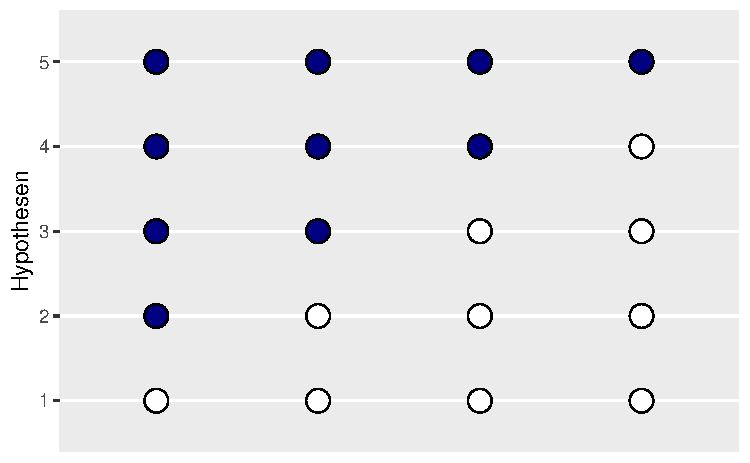
\includegraphics[width=0.2\linewidth]{unnamed-chunk-3-1} \end{figure}

(Kurz 2021)
\end{frame}

\begin{frame}{Unsere Daten}
\protect\hypertarget{unsere-daten}{}
\begin{itemize}
\tightlist
\item
  Wir ziehen eine Murmel, merken uns die Farbe und legen sie zurück. Das
  wiederholen wir noch zwei Mal (Ziehen mit Zurücklegen). Wir erhalten:
  BWB. Voilà: unsere Daten.
\end{itemize}

\begin{figure}[H]
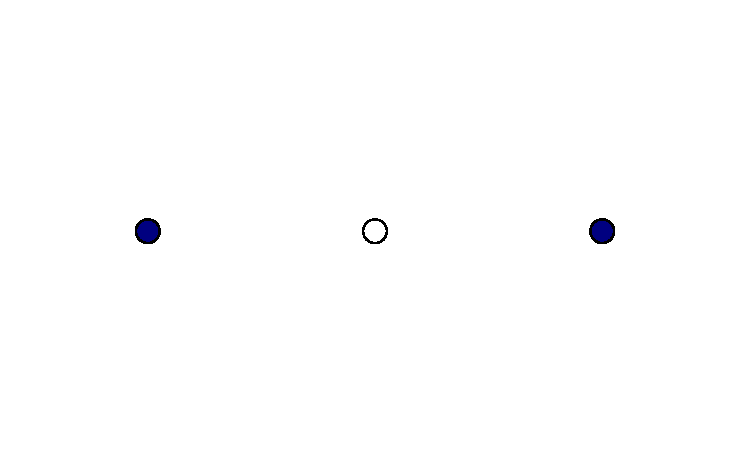
\includegraphics[width=0.7\linewidth]{unnamed-chunk-4-1} \end{figure}
\end{frame}

\begin{frame}{Zugmöglichkeiten laut Hypothese {[}BWWW{]}, 1. Zug}
\protect\hypertarget{zugmuxf6glichkeiten-laut-hypothese-bwww-1.-zug}{}
Wenn Hypothese {[}BWWW{]} der Fall sein sollte, dann können wir im
\emph{ersten} Zug entweder die eine blaue Murmel erwischen oder eine der
drei weißen.

\begin{figure}[H]
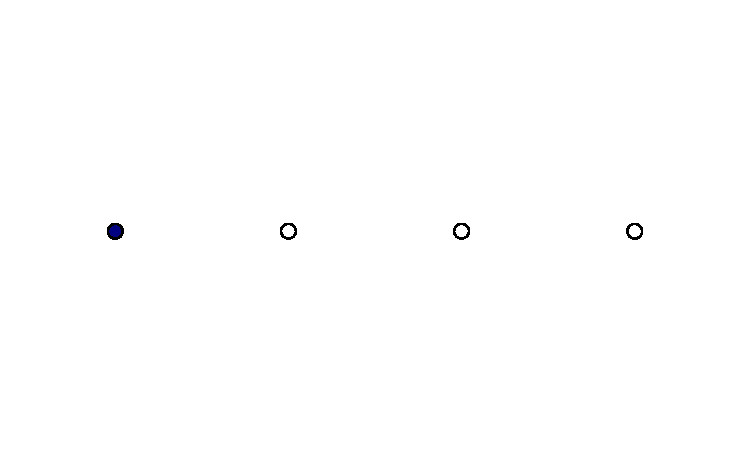
\includegraphics[width=0.5\linewidth]{unnamed-chunk-5-1} \end{figure}

Nachdem wir die Murmel gezogen haben (und die Farbe gemerkt haben),
legen wir sie wieder ins Säckchen: Ziehen mit Zurücklegen.
\end{frame}

\begin{frame}{Zugmöglichkeiten laut Hypothese {[}BWWW{]}, 1. und 2. Zug}
\protect\hypertarget{zugmuxf6glichkeiten-laut-hypothese-bwww-1.-und-2.-zug}{}
Wenn Hypothese {[}BWWW{]} der Fall sein sollte, dann haben wir im
\emph{zweiten} Zug natürlich die gleichen Möglichkeiten.

Zug 1 und Zug 2 zusammen genommen, gibt es also \(16=4\cdot4=4^2\)
Kombinationen, welche zwei Murmeln wir ziehen:

\begin{figure}[H]
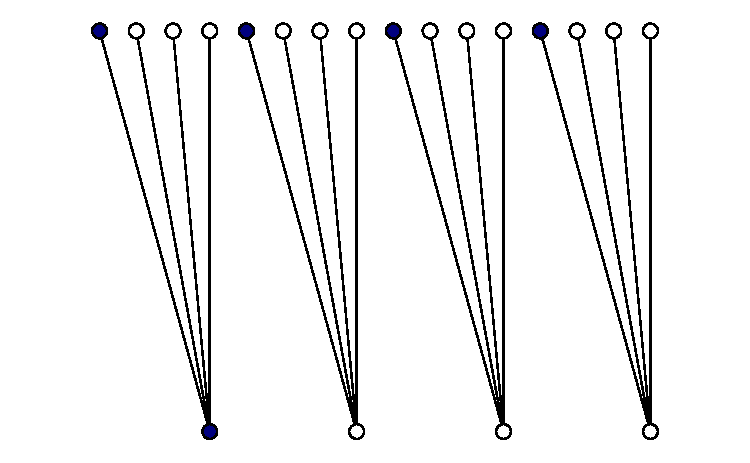
\includegraphics[width=0.5\linewidth]{unnamed-chunk-6-1} \end{figure}

Die ersten vier Kombinationen sind: BB, BW, BW, BW
\end{frame}

\begin{frame}{Zugmöglichkeiten laut Hypothese {[}BWWW{]}, 1.-3. Zug}
\protect\hypertarget{zugmuxf6glichkeiten-laut-hypothese-bwww-1.-3.-zug}{}
Zug 1, Zug 2 und Zug 3 zusammen genommen, gibt es dann
\(4\cdot4\cdot4=4^3=64\) Kombinationen, drei Murmeln zu ziehen.

\begin{figure}[H]
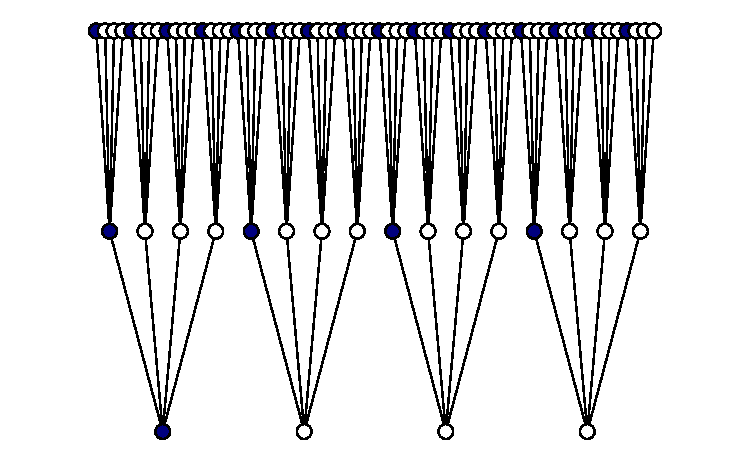
\includegraphics[width=0.5\linewidth]{unnamed-chunk-7-1} \end{figure}
\end{frame}

\begin{frame}{Welche Züge sind logisch möglich?}
\protect\hypertarget{welche-zuxfcge-sind-logisch-muxf6glich}{}
\begin{itemize}
\tightlist
\item
  Bei 3 Zügen (mit jeweils 4 möglichen Murmeln) gibt es \(4^3\)
  Kombinationen an Murmeln.
\item
  Aber einige Kombinationen lassen sich nicht mit unseren Daten (BWB)
  vereinbaren.
\item
  Z.B. alle Kombinationen die mit W beginnen, sind nicht mit unseren
  Daten zu vereinbaren, denn in unseren Daten ist die erste Murmel vom
  Typ B.
\end{itemize}

\begin{figure}[H]
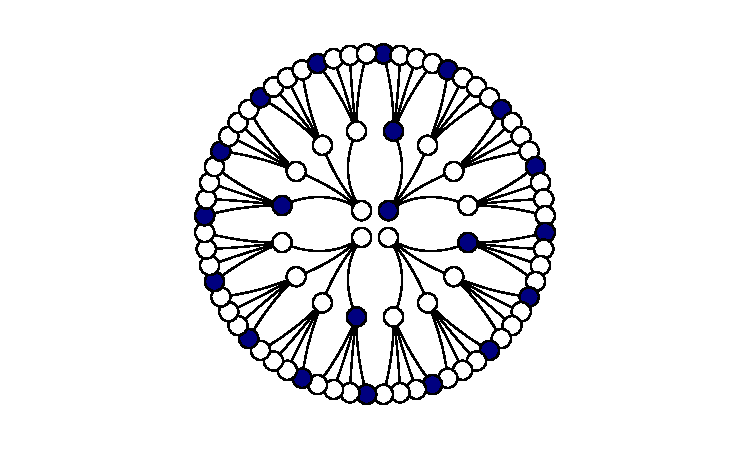
\includegraphics[width=0.49\linewidth]{unnamed-chunk-8-1} 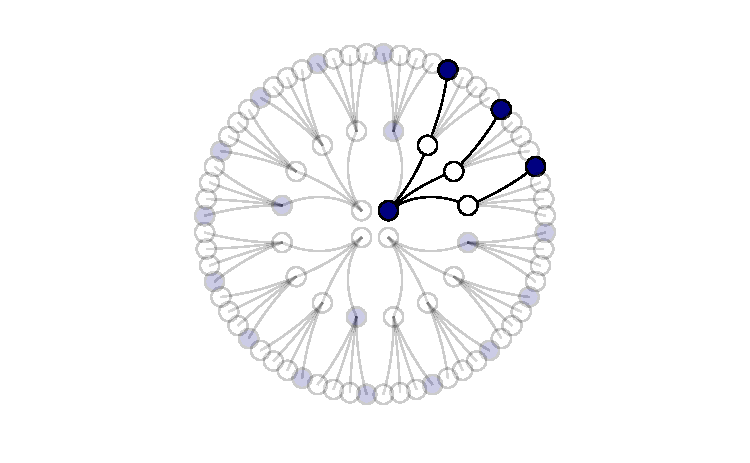
\includegraphics[width=0.49\linewidth]{unnamed-chunk-8-2} \end{figure}

Nur 3 der 64 ``Pfade'' (Kombinationen) sind mit unseren Daten logisch zu
vereinbaren.
\end{frame}

\begin{frame}{Kombinationen pro Hypothese}
\protect\hypertarget{kombinationen-pro-hypothese}{}
\begin{tabular}{l|l}
\hline
Hyp & Häufigkeit WBW\\
\hline
[W W W W] & 0 * 4 * 0 = 0\\
\hline
[B W W W] & 1 * 3 * 1 = 3\\
\hline
[B B W W] & 2 * 2 * 2 = 8\\
\hline
[B B B W] & 3 * 1 * 3 = 9\\
\hline
[B B B B] & 4 * 0 * 4 = 0\\
\hline
\end{tabular}

\begin{itemize}
\item
  Die Häufigkeiten der Kombinationen ist proportional zur Plausibilität
  einer Hypothese.
\item
  Zusätzlich müssten wir noch beachten, ob bestimmte Hypothesen
  \emph{per se} bzw. \emph{a priori} wahrscheinlicher sind. So könnten
  blaue Murmeln selten sein. Dann wäre die Hypothese {[}BBBB{]}
  entsprechend unwahrscheinlich.
\item
  Gehen wir der Einfachheit halber zunächst davon aus, dass alle
  Hypothesen apriori gleich wahrscheinlich sind.
\end{itemize}
\end{frame}

\begin{frame}{Pfadbaum für alle vier Hypothesen}
\protect\hypertarget{pfadbaum-fuxfcr-alle-vier-hypothesen}{}
\begin{figure}[H]
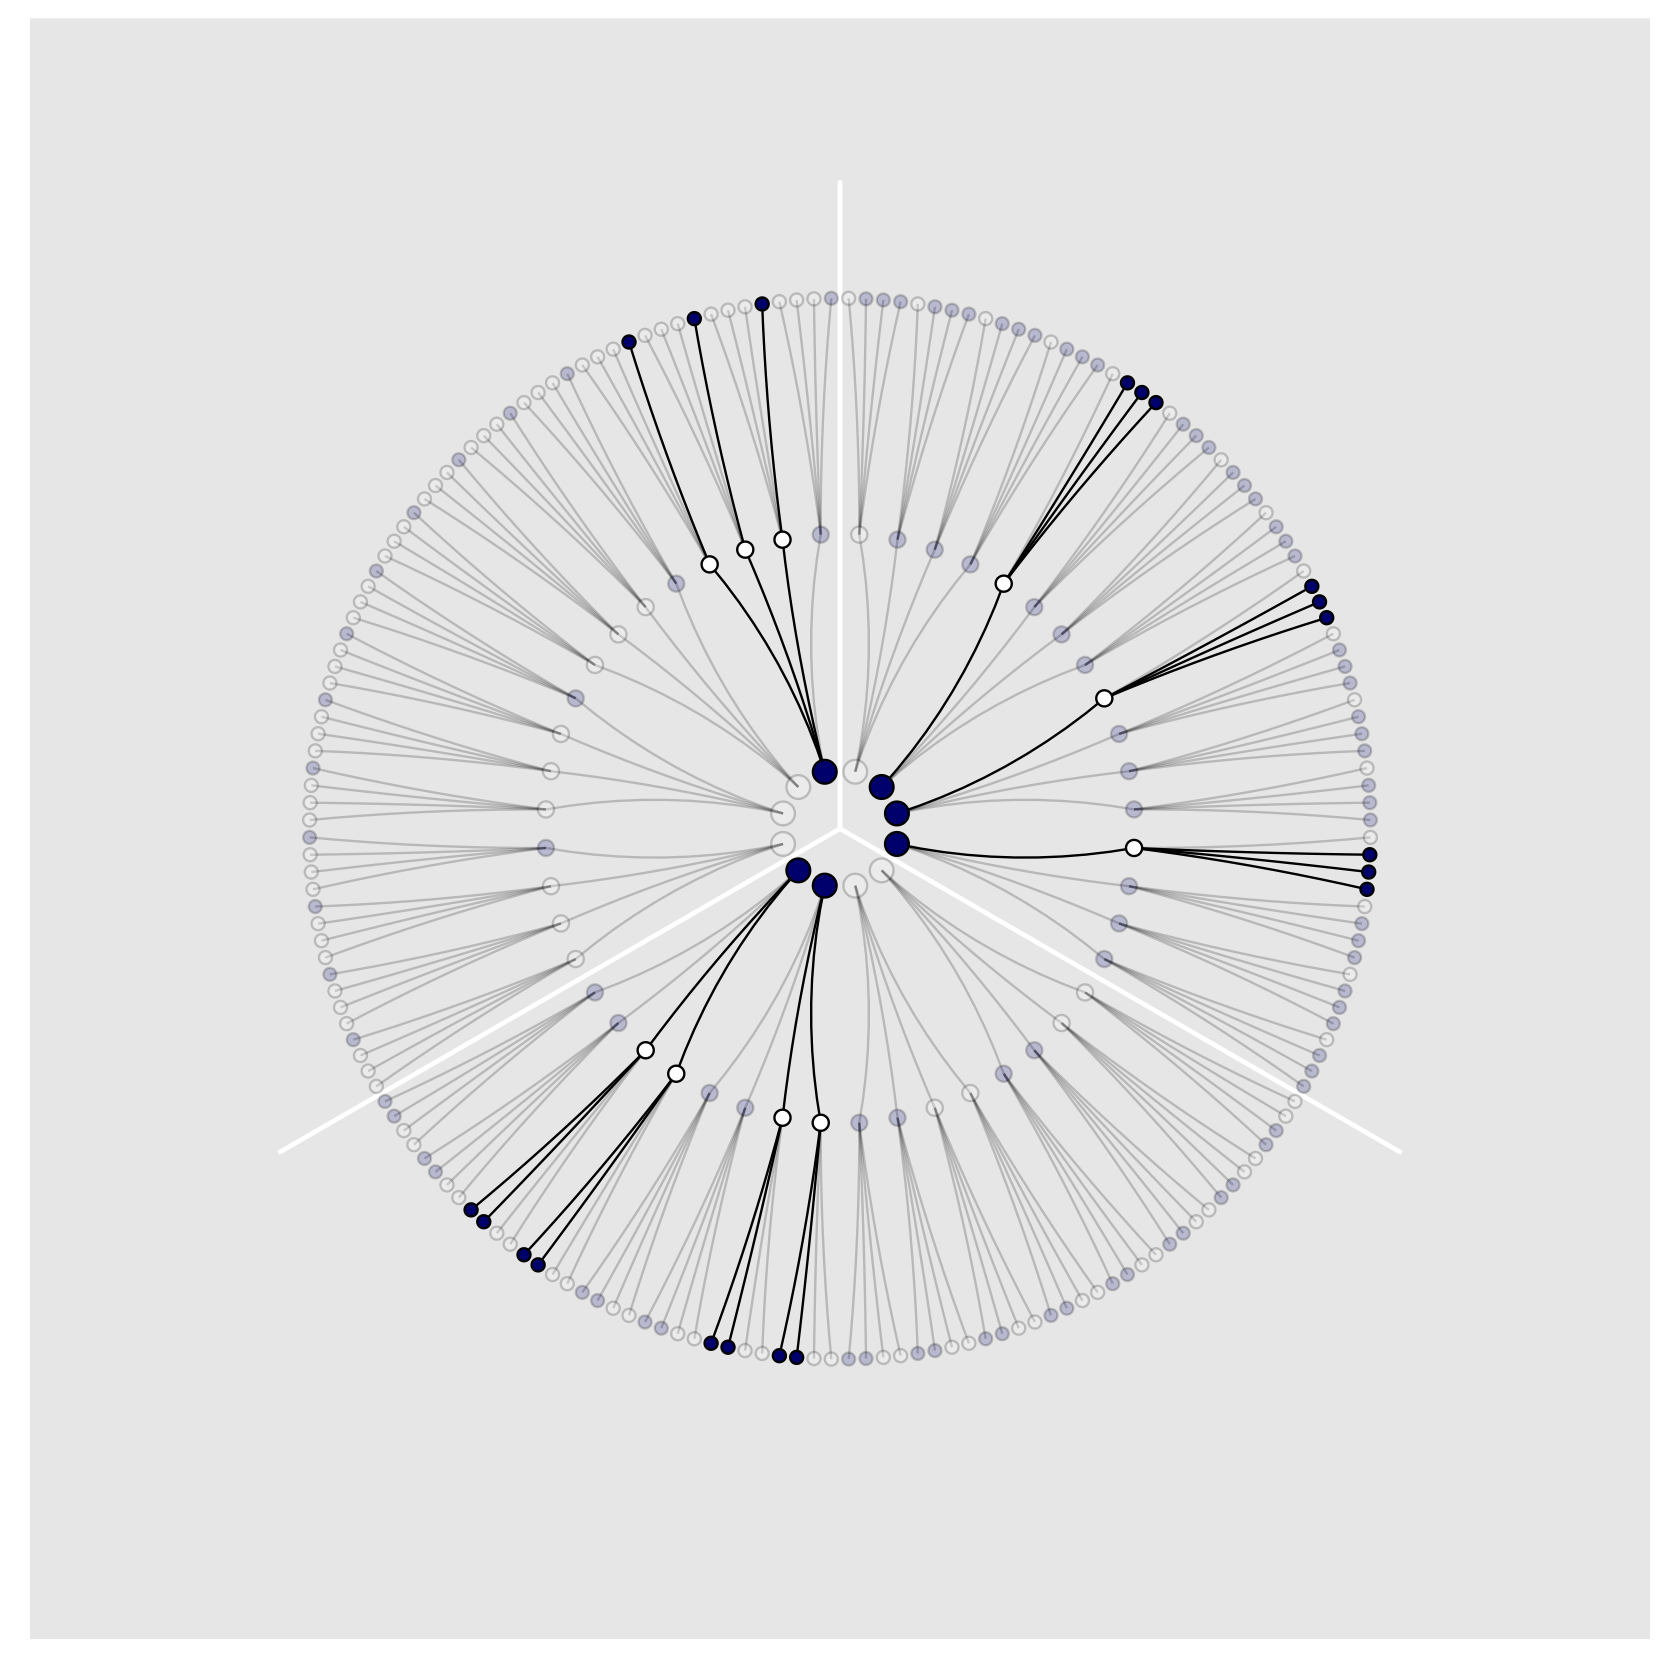
\includegraphics[width=0.7\linewidth]{img/img2118} \end{figure}
\end{frame}

\begin{frame}{Wir ziehen einer vierte Murmel: B}
\protect\hypertarget{wir-ziehen-einer-vierte-murmel-b}{}
\begin{itemize}
\tightlist
\item
  Gehen wir davon aus, dass alle Hypothesen apriori gleich
  wahrscheinlich sind.
\item
  Wir ziehen wieder eine Murmel. Sie ist blau (B)!
\item
  Jetzt könnten wir den Pfadbaum für vier (statt drei) Züge aufmalen.
\item
  Oder wir machen ein \emph{Update}: Wir aktualisieren die bisherigen
  Kombinationshäufigkeiten um die neuen Daten. Die \emph{alten} Daten
  dienen dabei als \emph{Priori-Informationen} für die \emph{neuen}
  Daten.
\end{itemize}
\end{frame}

\begin{frame}{Priori-Information nutzen}
\protect\hypertarget{priori-information-nutzen}{}
Mit den Daten BWBB ist die Hypothese {[}BBBW{]} am wahrscheinlichsten:

\begin{tabular}[t]{l|r|r|l}
\hline
Hyp & PB & HA & HN\\
\hline
[W W W W] & 0 & 0 & 0 * 0 = 0\\
\hline
[B W W W] & 1 & 3 & 1 * 3 = 3\\
\hline
[B B W W] & 2 & 8 & 2 * 8 = 16\\
\hline
[B B B W] & 3 & 9 & 3 * 9 = 27\\
\hline
[B B B B] & 4 & 0 & 4 * 0 = 0\\
\hline
\end{tabular}

Hyp: Hypothese

PB: Anzahl von Pfaden für B

HA: alte (bisherige) Häufigkeiten

HN: neue (geupdatete) Häufigkeiten
\end{frame}

\begin{frame}{Murmelfabrik streikt: Blaue Murmeln jetzt sehr selten!}
\protect\hypertarget{murmelfabrik-streikt-blaue-murmeln-jetzt-sehr-selten}{}
\begin{itemize}
\item
  Berücksichtigen wir die Information, dass apriori (bevor wir die Daten
  gesehen haben), einige Hypothesen wahrscheinlicher (plausibler) sind.
\item
  Dann ist die Hypothese {[}BBWW{]} am wahrscheinlichsten.
\end{itemize}

\begin{tabular}{l|r|r|l}
\hline
Hyp & HA & HF & HN\\
\hline
[W W W W] & 0 & 0 & 0 * 0 = 0\\
\hline
[B W W W] & 3 & 3 & 3 * 3 = 9\\
\hline
[B B W W] & 16 & 2 & 16 * 2 = 32\\
\hline
[B B B W] & 27 & 1 & 27 * 1 = 27\\
\hline
[B B B B] & 0 & 0 & 0 * 0 = 0\\
\hline
\end{tabular}

HF: Häufigkeit des Säckchentyps laut Fabrik
\end{frame}

\begin{frame}{Zählen mit großen Zahlen nervt}
\protect\hypertarget{zuxe4hlen-mit-grouxdfen-zahlen-nervt}{}
\begin{itemize}
\item
  Malen Sie mal den Pfadbaum für 10 Züge \ldots{}
\item
  Eine Umrechnung der Häufigkeiten in \emph{Anteile} macht das Rechnen
  einfacher.
\item
  Dazu definieren wir die \emph{geupdatete Plausibilität einer Hypothese
  nach Kenntnis der Daten}:
\end{itemize}

\[\text{Plausibilität von [BWWW] nach Kenntnis von BWB}\] \[\propto\]
\[\text{Anzahl möglicher Pfade bei [BWWWW] für BWB}\] \[\times\]
\[\text{Priori-Plausibilität von [BWWWW]}\]

\begin{itemize}
\tightlist
\item
  \(\propto\): proportional zu
\end{itemize}
\end{frame}

\begin{frame}{Plausibilität berechnen}
\protect\hypertarget{plausibilituxe4t-berechnen}{}
\begin{itemize}
\item
  Sei \(p\) der Anteil blauer Murmeln. Bei Hypothese {[}BWWW{]} gilt
  dann: \(p=1/4 = 0.25\). Sei \(D_{neu} =\) BWB, die Daten.
\item
  Es gilt:
\end{itemize}

\[\text{Plausibilität von }p\text{ nach Kenntnis von }D_{neu}\]
\[\propto\] \[\text{Anzahl Pfade von }p\text{ für }D_{neu}\] \[\times\]
\[\text{Priori-Plausibilität von }p\]

``Für jeden Wert von \(p\) beurteilen wir dessen Plausibilität als umso
höher (proportional), je mehr Pfade durch den Pfadbaum führen.''
\end{frame}

\begin{frame}{Von Plausibilität zur Wahrscheinlichkeit}
\protect\hypertarget{von-plausibilituxe4t-zur-wahrscheinlichkeit}{}
\begin{itemize}
\tightlist
\item
  Teilen wir die Anzahl Pfade einer Hypothese durch die Anzahl aller
  Pfade (aller Hypothesen), so bekommen wir einen Anteil. Damit haben
  wir eine Wahrscheinlichkeit:
\end{itemize}

\[\text{Pl von }p\text{mit Daten }D_{neu} =\]
\[\frac{\text{Anzahl Pfade von }p\text{ für }D_{neu}\times \text{Prior-Pl von }p}{\text{Summe aller Pfade}}\]

Pl: Plausibilität
\end{frame}

\begin{frame}[fragile]{Plausibilität pro Hypothese}
\protect\hypertarget{plausibilituxe4t-pro-hypothese}{}
\begin{tabular}{l|r|r|r}
\hline
Hyp & p & AP & Pl\\
\hline
[W W W W] & 0.00 & 0 & 0.00\\
\hline
[B W W W] & 0.25 & 3 & 0.15\\
\hline
[B B W W] & 0.50 & 8 & 0.40\\
\hline
[B B B W] & 0.75 & 9 & 0.45\\
\hline
[B B B B] & 1.00 & 0 & 0.00\\
\hline
\end{tabular}

p: Anteil blauer Murmeln (Priori-Information)

AP: Anzahl von möglichen Pfaden

Pl: Plausibilität

\begin{Shaded}
\begin{Highlighting}[]
\NormalTok{AP }\OtherTok{\textless{}{-}} \FunctionTok{c}\NormalTok{(}\DecValTok{0}\NormalTok{, }\DecValTok{3}\NormalTok{, }\DecValTok{8}\NormalTok{, }\DecValTok{9}\NormalTok{, }\DecValTok{0}\NormalTok{)}
\NormalTok{Pl }\OtherTok{\textless{}{-}}\NormalTok{ AP }\SpecialCharTok{/} \FunctionTok{sum}\NormalTok{(AP)}
\NormalTok{Pl}
\end{Highlighting}
\end{Shaded}

\begin{verbatim}
## [1] 0.00 0.15 0.40 0.45 0.00
\end{verbatim}
\end{frame}

\begin{frame}{Fachbegriffe}
\protect\hypertarget{fachbegriffe}{}
\begin{itemize}
\item
  Kennwerte laut einer Hypothese, wie den Anteil blauer Murmeln \(p\)
  bezeichnet man als \emph{Parameter}.
\item
  Den Anteil gültiger Pfade pro Hypothese (bzw. pro \(p\)) bezeichnet
  man als \emph{Likelihood}.
\item
  Die Priori-Plausibilität nennt man \emph{Priori-Wahrscheinlichkeit}.
\item
  Die neue, geupdatete Plausibilität für einen bestimmten Wert von \(p\)
  nennt man \emph{Posteriori-Wahrscheinlichkeit}.
\end{itemize}
\end{frame}

\hypertarget{hinweise}{%
\section{Hinweise}\label{hinweise}}

\begin{frame}{Lehrbuch und Homepage des Lehrbuchs}
\protect\hypertarget{lehrbuch-und-homepage-des-lehrbuchs}{}
Dieses Skript bezieht sich auf folgende
\protect\hyperlink{literatur}{Lehrbücher}:

\begin{itemize}
\tightlist
\item
  Kapitel 2 aus McElreath (2016) (``ReThink\_v1'')
\item
  R-Code für die Diagramme stammt aus Kurz (2021)
\end{itemize}
\end{frame}

\begin{frame}{Literatur}
\protect\hypertarget{literatur}{}
\hypertarget{refs}{}
\begin{CSLReferences}{1}{0}
\leavevmode\vadjust pre{\hypertarget{ref-kurz_statistical_2021}{}}%
Kurz, A. Solomon. 2021. \emph{Statistical Rethinking with Brms, Ggplot2,
and the Tidyverse: {Second} Edition}.
\url{https://bookdown.org/content/4857/}.

\leavevmode\vadjust pre{\hypertarget{ref-McElreath2016}{}}%
McElreath, Richard. 2016. \emph{Statistical {Rethinking}}. 1. Aufl. {New
York City, NY}: {CRC Press}.

\end{CSLReferences}
\end{frame}

\end{document}
